\documentclass{article}
\usepackage[utf8]{inputenc}
\usepackage{amsmath}
\usepackage{amsfonts}
\usepackage{amssymb}
\usepackage{graphicx}											% Use pdf, png, jpg, or eps§ with pdflatex; use eps in DVI
\usepackage[left=2cm, right=2cm, top=2cm, bottom=2cm]{geometry}
\usepackage{float}													% for controlling the position of objects ie. tables

\usepackage[small, bf]{caption}								%Adjust caption size of figures, tables, pictures...
\setlength{\captionmargin}{15pt}
										
\graphicspath{{images/}}				% folder where images are stored in current directory


% --------------------------- Code for placing two figure side by side ---------------------------------------------------------------------------------
\usepackage{caption}
\usepackage{subcaption}

% --------------------------- Code for the bibliography ---------------------------------------------------------------------------------
\usepackage{natbib}												% For fancy in-text citations
\bibliographystyle{plain}

\author{Curtis Rau}
\title{A C++ Implementation of the Thomas Algorithm to Solve the One Dimensional Poisson Equation}


\begin{document}

\maketitle

\begin{abstract}
In this project we sought to implement the Thomas Algorithm, which is a LU decomposition method for solving tridiagonal matricies, to solve the Poisson Equation with Dirichlet boundary conditions.  In short, the equation to be solved is a non-homogenious second order linear partial differential equation.  We discretize the equation, which generates a system of equations, but because the differential equation is linear, this discretized system of equations is also linear, so it can be expressed as a matrix equation of the form Ax=b.  The matrix A is tridiagonal.  Gaussian elimination can be used to solve the system ($\propto N^3$ flops) but a much faster method of solving the system is the Thomas Algorithm ($\propto N$ flops).
\end{abstract}

%\begin{multicols}{2}

\section{Motivation}
The Poisson Equation is a partial differential equation of the form

\begin{equation}
	- \frac{\partial^2 u}{\partial x^2} = f(x)
\end{equation}

which comes up often in physics.  One such application is Gauss’s Law in differential form.  To find a numerical solution to Poisson’s Equation we discretize x

\begin{equation}
\begin{aligned}
	x    &\to & x_i          \\
	u(x) &\to & u(x_i) = u_i \\
	f(x) &\to & f(x_i) = f_i
\end{aligned}
\end{equation}

and we utilize the limit definition of the second derivative

\begin{equation}
	\frac{\partial^2 u}{\partial x^2} = \lim_{N \to \infty} \frac{u_{i-1} - 2 u_i + u_{i+1}}{h^2}
\end{equation}

where $h = x_{i+1} - x_i = $ (length) / (number of divisions).  The discretized Poisson’s Equation reads

\begin{equation}
\begin{aligned}
	\frac{u_{i-1} - 2 u_i + u_{i+1}}{h^2} = - f_i \\
	- u_{i-1} + 2 u_i - u_{i+1} = h^2 f_i
\end{aligned}
\end{equation}

As the number of divisions increases the numerical results will converge to the analytical result.  We can now write this as a system of linear equations:

\begin{equation} 
\begin{aligned}
                            u_1 &=& uFirst      \\
            - u_1 + 2 u_2 - u_3 &=& h^2 f_2     \\
            - u_2 + 2 u_3 - u_4 &=& h^2 f_3     \\
                             &\vdots &          \\
- u_{N-3} + 2 u_{N-2} - u_{N-1} &=& h^2 f_{N-2} \\
    - u_{N-2} + 2 u_{N-1} - u_N &=& h^2 f_{N-1} \\
                            u_N &=& uLast
\end{aligned} 
\end{equation}

The first and last equations are the boundary conditions.  There are N equations and N unknowns, so this linear system has only one solution.  The language of C++, in which the program was written, has the interesting (read frustrating and unintuitive) property that counting starts with 0.  So before we proceed we should make the indicies of the arrays f and u start with 0 so

\begin{equation}
\begin{aligned}
	f_i &\to f_{i-2} \\
	u_i &\to u_{i-1}
\end{aligned}
\end{equation}


The endpoints, $u_0$ and $u_N$, are already known (because of boundary conditions) so we can remove the first and last equation from the system.  By rearranging the second and second to last equation we can arrive at a suggestive form for the system.  In the following equation, blank spots within the matrix represent 0's, and were ommitted so as to highlight the structure of the sparse matrix.

\begin{equation}
\label{eqn: mat system}
\left( \begin{array}{ccccc}
	 2 & -1 &        &    &    \\
	-1 &  2 &   -1   &    &    \\
	   &    & \ddots &    &    \\
	   &	    &   -1   &  2 & -1 \\
	   &    &        & -1 &  2
   \end{array} \right)
\left( \begin{array}{c}
	u_1     \\
	u_2     \\
	\vdots  \\
	u_{N-3} \\
	u_{N-2}
   \end{array} \right)
=
\left( \begin{array}{c}
	h^2 f_0 + u_0     \\
	h^2 f_1           \\
	\vdots        \\
	h^2 f_{N-4}       \\
	h^2 f_{N-3} + u_{N-1} \\
   \end{array} \right)
\end{equation}

We can append the endpoints to the solution array after the program has run if we so desire.

\section{The Thomas Algorithm}
To solve equation \ref{eqn: mat system} we use the Thomas Algorithm.  A theorm of Linear Algebra states that any matrix can be decomposed into a product of an upper and lower triangular matrix.  The Thomas Algorithm is a LU Decomposition algorithm that is equivalent to a Gaussian Elimination algorithm.  First consider the general $m\times m$ tridiagonal matrix system.

\begin{equation}
\label{eqn: mat system}
\left( \begin{array}{ccccc}
	 b0 & c0 &        &         &         \\
	a0 &  b1 &  c1    &         &         \\
	   &    & \ddots  &         &         \\
	   &	    & a_{m-3} & b_{m-2} & c_{m-2} \\
	   &    &         & a_{m-2} & b_{m-1}
   \end{array} \right)
\left( \begin{array}{c}
	x_0     \\
	x_1     \\
	\vdots  \\
	x_{m-2} \\
	x_{m-1}
   \end{array} \right)
=
\left( \begin{array}{c}
	g_0     \\
	g_1     \\
	\vdots  \\
	g_{m-2} \\
	g_{m-1} \\
   \end{array} \right)
\end{equation}

The first step is to multiply the first row by a0/b0 and subtract it from the second row.  This is known as the forward substitution step.  By itterating this step the a's are eliminated, leaving an upper triangular matrix.

\begin{equation}
\begin{aligned}
	a_i &=& 0                                    \\
	b_i &=& b_i - \frac{a_{i-1}}{b_{i-1}}c_{i-1} \\
	g_i &=& g_i - \frac{a_{i-1}}{b_{i-1}}g_{i-1}
\end{aligned}
\end{equation}

At this point the simplified equation, with only an upper triangular matrix takes the form

\begin{equation}
\label{eqn: mat system}
\left( \begin{array}{ccccc}
    b0 & c0 &        &         &         \\
	   & b1 &  c1    &         &         \\
	   &    & \ddots &         &         \\
	   &	    &        & b_{m-2} & c_{m-2} \\
	   &    &        &         & b_{m-1}
   \end{array} \right)
\left( \begin{array}{c}
	x_0     \\
	x_1     \\
	\vdots  \\
	x_{m-2} \\
	x_{m-1}
   \end{array} \right)
=
\left( \begin{array}{c}
	g_0     \\
	g_1     \\
	\vdots  \\
	g_{m-2} \\
	g_{m-1} \\
   \end{array} \right)
\end{equation}

Now for the backwards substitution step.  The last row is multiplied by $c_{N-3}/b_{N-2}$ and subtracted from the second to last row, thus eliminating $c_{N-3}$ from the last row.  The general backwards substitution procedure is 

\begin{equation}
\begin{aligned}
	c_i &=& 0                                    \\
	g_{i-1} &=& g_{i-1} - \frac{c_{i-1}}{b_i}g_i
\end{aligned}
\end{equation}

Iterating this process over the remaining c’s leaves a diagonal matrix

\begin{equation}
\label{eqn: mat system}
\left( \begin{array}{ccccc}
    b0 &    &        &         &         \\
	   & b1 &        &         &         \\
	   &    & \ddots &         &         \\
	   &	    &        & b_{m-2} &         \\
	   &    &        &         & b_{m-1}
   \end{array} \right)
\left( \begin{array}{c}
	x_0     \\
	x_1     \\
	\vdots  \\
	x_{m-2} \\
	x_{m-1}
   \end{array} \right)
=
\left( \begin{array}{c}
	g_0     \\
	g_1     \\
	\vdots  \\
	g_{m-2} \\
	g_{m-1} \\
   \end{array} \right)
\end{equation}

All that ramains to be computed is the solution, which is the very straight forward process of

\begin{equation}
x_i = \frac{f_i}{b_i}
\end{equation}

The function I wrote to perform this algorithim is displayed below.  It takes pointers to a, b, c, u, and f -- the vectors; and a integer N to tell the function how long the vectors are for the for loops.  The indicies of the u vector are shifted up one so that the endpoints can be assigned.

\begin{figure}[H]
	\centering
	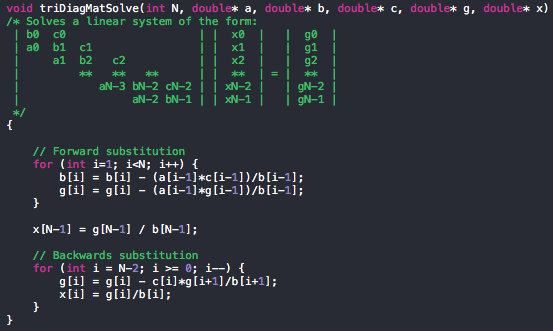
\includegraphics[width=0.8\linewidth]{cppThomasAlgorithm.png}
	\caption{}
\end{figure}

A summery of the opperations the processor has to perform for this algorithm are given below.

\begin{table}[H]
	\centering
	\begin{tabular}{ c | c | c }
		Operation	    & Floating Point & Integer          \\
		\hline
		Memory Reads    &    $14(N-2)$   & $18(N-2)$        \\
		\hline
		Memory Writes   &     $4(N-2)$   & $2(N-1)$         \\
		\hline
		Additions       &                & $3(N-2) + (N-1)$ \\
		\hline
		Subtractions    &     $3(N-2)$   & $7(N-2) + (N-1)$ \\
		\hline
		Multiplications &     $3(N-2)$   &                  \\
		\hline
		Divisions       &     $4(N-2)$   &		           \\
		\hline
		Comparisons	    &                & $2(N-1)$         \\
	\end{tabular}
	\caption{ \label{table:}}
\end{table}

\section{Faster, Tuned Algorithms}
The generality of the Thomas Algorithm is unnecessary for the problem at hand.  Using it to solve the Poisson Equation means $a=c=1$ and $b=-2$.  Additionally we are using dirichlet boundary conditions so calculating the f vector can be somewhat simplified.  Further simplification can be realized by recognizing the recursive relation for $b$ given in equation (9) can be expressed in explicit form:

\begin{equation}
b_i = \frac{i+2}{i+1}
\end{equation}

The implementation of this looks like:

\begin{figure}[H]
	\centering
	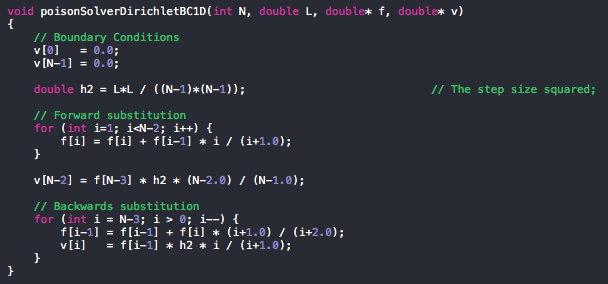
\includegraphics[width=0.8\linewidth]{cppPoissonSolverFast.png}
	\caption{}
\end{figure}



\section{Results}
The benchmarks for the three solving methods is given by the following table.

\begin{table}[H]
	\centering
	\begin{tabular}{ c | c | c | c }
		N      &  Thomas Algorithm    &       Thomas Algorithm      & Optimized Algorithm  \\
		       &  Computation Time    & Computation Time (Adjusted) &  Computation Time    \\
		\hline
		5      & $4.7 \cdot 10^{-5}$  &     $3.5 \cdot 10^{-5}$     & $3.3 \cdot 10^{-5}$  \\
		\hline
		10     & $3.5 \cdot 10^{-5}$  &     $3.5 \cdot 10^{-5}$     & $3.3 \cdot 10^{-5}$  \\
		\hline
		25     & $3.5 \cdot 10^{-5}$  &     $3.5 \cdot 10^{-5}$     & $3.5 \cdot 10^{-5}$  \\
		\hline
		100    & $7.3 \cdot 10^{-5}$  &     $4.1 \cdot 10^{-5}$     & $3.7 \cdot 10^{-5}$  \\
		\hline
		1,000  & $7.0 \cdot 10^{-5}$  &     $9.4 \cdot 10^{-5}$     & $6.9 \cdot 10^{-5}$  \\
		\hline
		10,000 & $4.06 \cdot 10^{-4}$ &     $6.05 \cdot 10^{-4}$    & $3.79 \cdot 10^{-4}$
	\end{tabular}
	\caption{ \label{table:}}
\end{table}

The code was benchmarked on a macbook pro.  Apple’s Grand Central Dispatch (GCD) makes accurately benchmarking almost impossible.  The way this code is written it will execute on one thread.  Modern operating systems break up thread execution because there are almost always more threads executing at any given time than there are cores in the processor.  This means the execution time as shown above is probably a factor of 10 to 100 times longer than if the thread were to execute continuously.  All that can be done on a computer running a modern operating system (without fancy code or dedicated cores) is set an upper limit on the computation time.  This also makes it difficult to empirically verify the dependency of computation time on the number of points.  Running identical code two times commonly yealds two distinct computation times.  The ones shown in the table above represent the smallest time observed.

The equation we tested these algorithms on is

\begin{equation}
- \frac{\partial^2 u}{\partial x^2} = 100 e^{-10x}
\end{equation}

with Dirichlet boundary conditions the solution is

\begin{equation}
u(x) = 1 - \left( 1 - e^{-10} \right) x - e^{-10x}
\end{equation}

Numerical approximations with increasing number of points are given below.

\begin{figure}[H]
	\centering
	\begin{subfigure}{.5\textwidth}
  		\centering
  		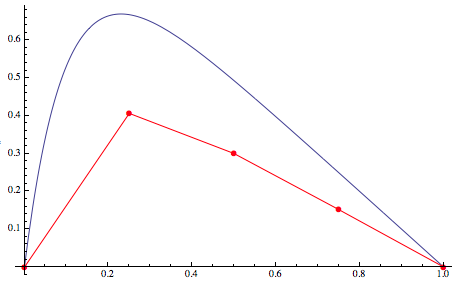
\includegraphics[width=.9\linewidth]{solutionN5}
  		\caption{Numerical solution with 5 interior points. \label{fig: hermite gaussian modes}}
	\end{subfigure}%
	\begin{subfigure}{.5\textwidth}
  		\centering
  		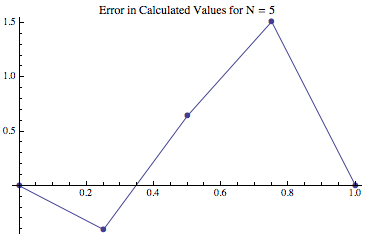
\includegraphics[width=.9\linewidth]{solutionErrorN5}
  		\caption{Laguerre Gaussian Modes \label{fig:  laguerre gaussian modes}}
	\end{subfigure}
	
%	\caption{A figure with two subfigures}
\end{figure}


\begin{figure}[H]
	\centering
	\begin{subfigure}{.5\textwidth}
  		\centering
  		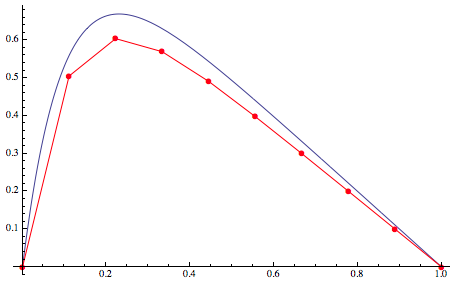
\includegraphics[width=.9\linewidth]{solutionN10}
  		\caption{Numerical solution with 10 interior points. \label{fig: }}
	\end{subfigure}%
	\begin{subfigure}{.5\textwidth}
  		\centering
  		\includegraphics[width=.9\linewidth]{solutionErrorN10}
  		\caption{Point by point error in numerical solution with 10 interior points \label{fig: }}
	\end{subfigure}
\end{figure}


\begin{figure}[H]
	\begin{subfigure}{.5\textwidth}
  		\centering
  		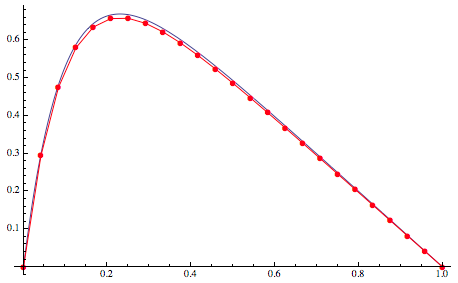
\includegraphics[width=.9\linewidth]{solutionN25}
  		\caption{Numerical solution with 25 interior points. \label{fig: }}
	\end{subfigure}%
	\begin{subfigure}{.5\textwidth}
  		\centering
  		\includegraphics[width=.9\linewidth]{solutionErrorN25}
  		\caption{Point by point error in numerical solution with 25 interior points \label{fig: }}
	\end{subfigure}

%	\caption{A figure with two subfigures}
\end{figure}
	
\begin{figure}[H]
	\centering
	
	\begin{subfigure}{.5\textwidth}
  		\centering
  		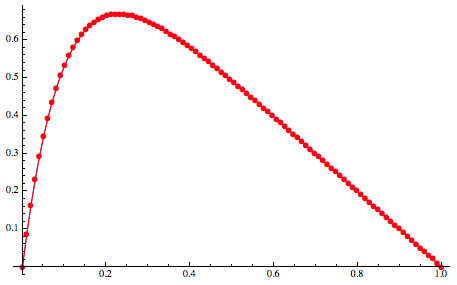
\includegraphics[width=.9\linewidth]{solutionN100}
  		\caption{Numerical solution with 100 interior points. \label{fig: }}
	\end{subfigure}%
	\begin{subfigure}{.5\textwidth}
  		\centering
  		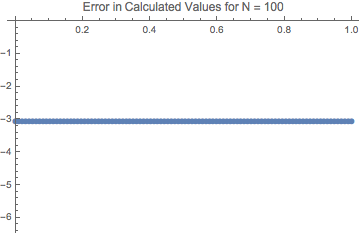
\includegraphics[width=.9\linewidth]{solutionErrorN100}
  		\caption{Point by point error in numerical solution with 100 interior points \label{fig: }}
	\end{subfigure}
	\caption{These calculated error graphs look pretty suspicious to me.  I’m going to take a closer look at them.  Namely ther error is clearly going to zero, but errors, indicated by the error graphs, are not going down, rather the shape is converging to something unexpected.}
\end{figure}

\end{document}